%!TEX TS-program = xelatex
%!TEX encoding = UTF-8 Unicode
\documentclass[12pt,a4paper]{article}
\usepackage{geometry} % 設定邊界
\geometry{
  top=1in,
  inner=1in,
  outer=1in,
  bottom=1in,
  headheight=3ex,
  headsep=2ex
}
\usepackage{fontspec} % 允許設定字體
\usepackage{xeCJK} % 分開設置中英文字型
\setCJKmainfont{LiHei Pro} % 設定中文字型
\setmainfont{Georgia} % 設定英文字型
\setromanfont{Georgia} % 字型
\setmonofont{Courier New}
\linespread{1.2}\selectfont % 行距
\XeTeXlinebreaklocale "zh" % 針對中文自動換行
\XeTeXlinebreakskip = 0pt plus 1pt % 字與字之間加入0pt至1pt的間距,確保左右對整齊
\parindent 0em % 段落縮進
\setlength{\parskip}{20pt} % 段落之間的距離

\title{\huge 資訊安全作業 Assignment1} % 設置標題,使用巨大字體
\author{吳嘉偉 5105056013} % 設置作者
\date{2017/03/26} % 設置日期
\usepackage{titling}
\setlength{\droptitle}{-8em} % 將標題移動至頁面的上面
\usepackage{listings}

\begin{document}

\clearpage

\maketitle % 顯示標題

\section{安裝Python Packages}

\subsection{使用終端機安裝pip}

{
\fontsize{14pt}{10pt} % 字型大小14pt,字行間距20pt
\selectfont % 生效
打開terminal後,先輸入指令安裝pip
\newline sudo easy\_install pip

\begin{figure}[ht]
	\begin{center}
		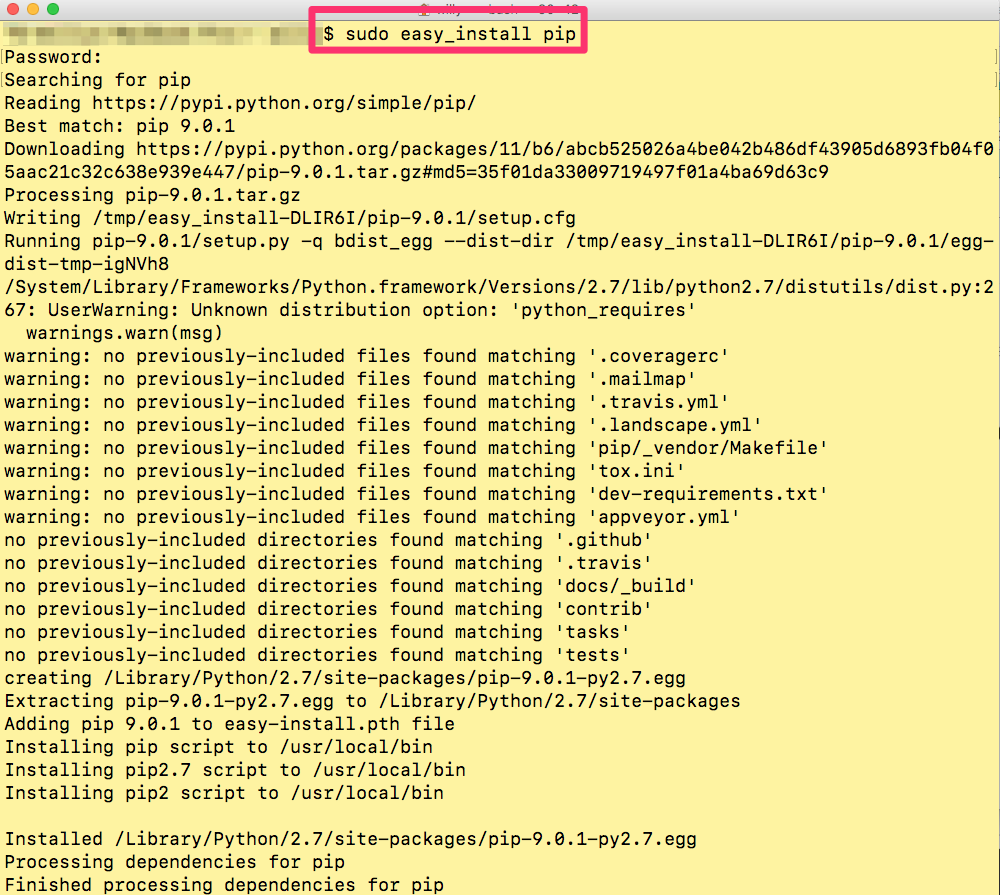
\includegraphics[scale=0.3]{image/termanal1.png}
		\caption{安裝pip}
	\end{center}
\end{figure}

\newpage % 新一頁
接著輸入下圖指令,安裝需要的package
\newline 這邊是安裝cryptography,版本為1.8.1
\newline sudo pip install packagename==version
\newline packagename:要安裝的package名稱
\newline version:要安裝的版本號碼

\begin{figure}[ht]
	\begin{center}
		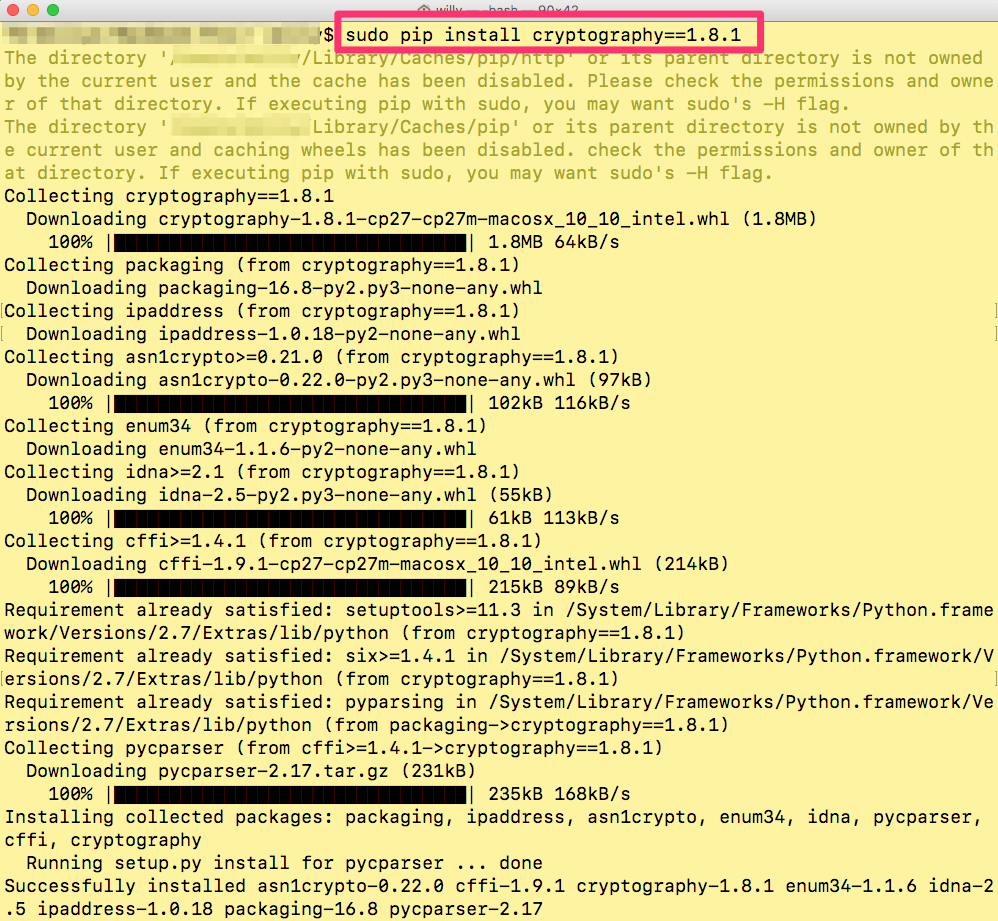
\includegraphics[scale=0.3]{image/termanal2.png}
		\caption{安裝package}
	\end{center}
\end{figure}
}

\subsection{使用PyCharm}

{
\fontsize{14pt}{10pt} % 字型大小12pt,字行間距10pt
\selectfont % 生效
打開PyCharmCE,先點選Preferences…

\begin{figure}[ht]
	\begin{center}
		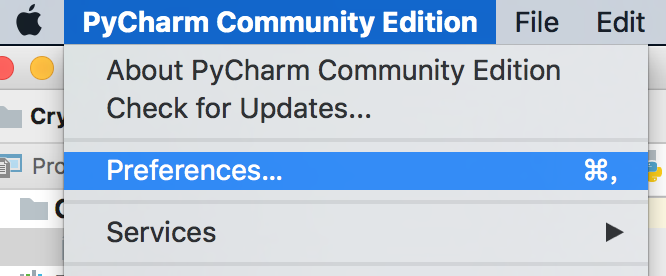
\includegraphics[scale=0.3]{image/PyCharm1.png}
	\end{center}
\end{figure}

\newpage % 新一頁
選擇Project: ProjectName >> Project Interpreter >> +

\begin{figure}[ht]
	\begin{center}
		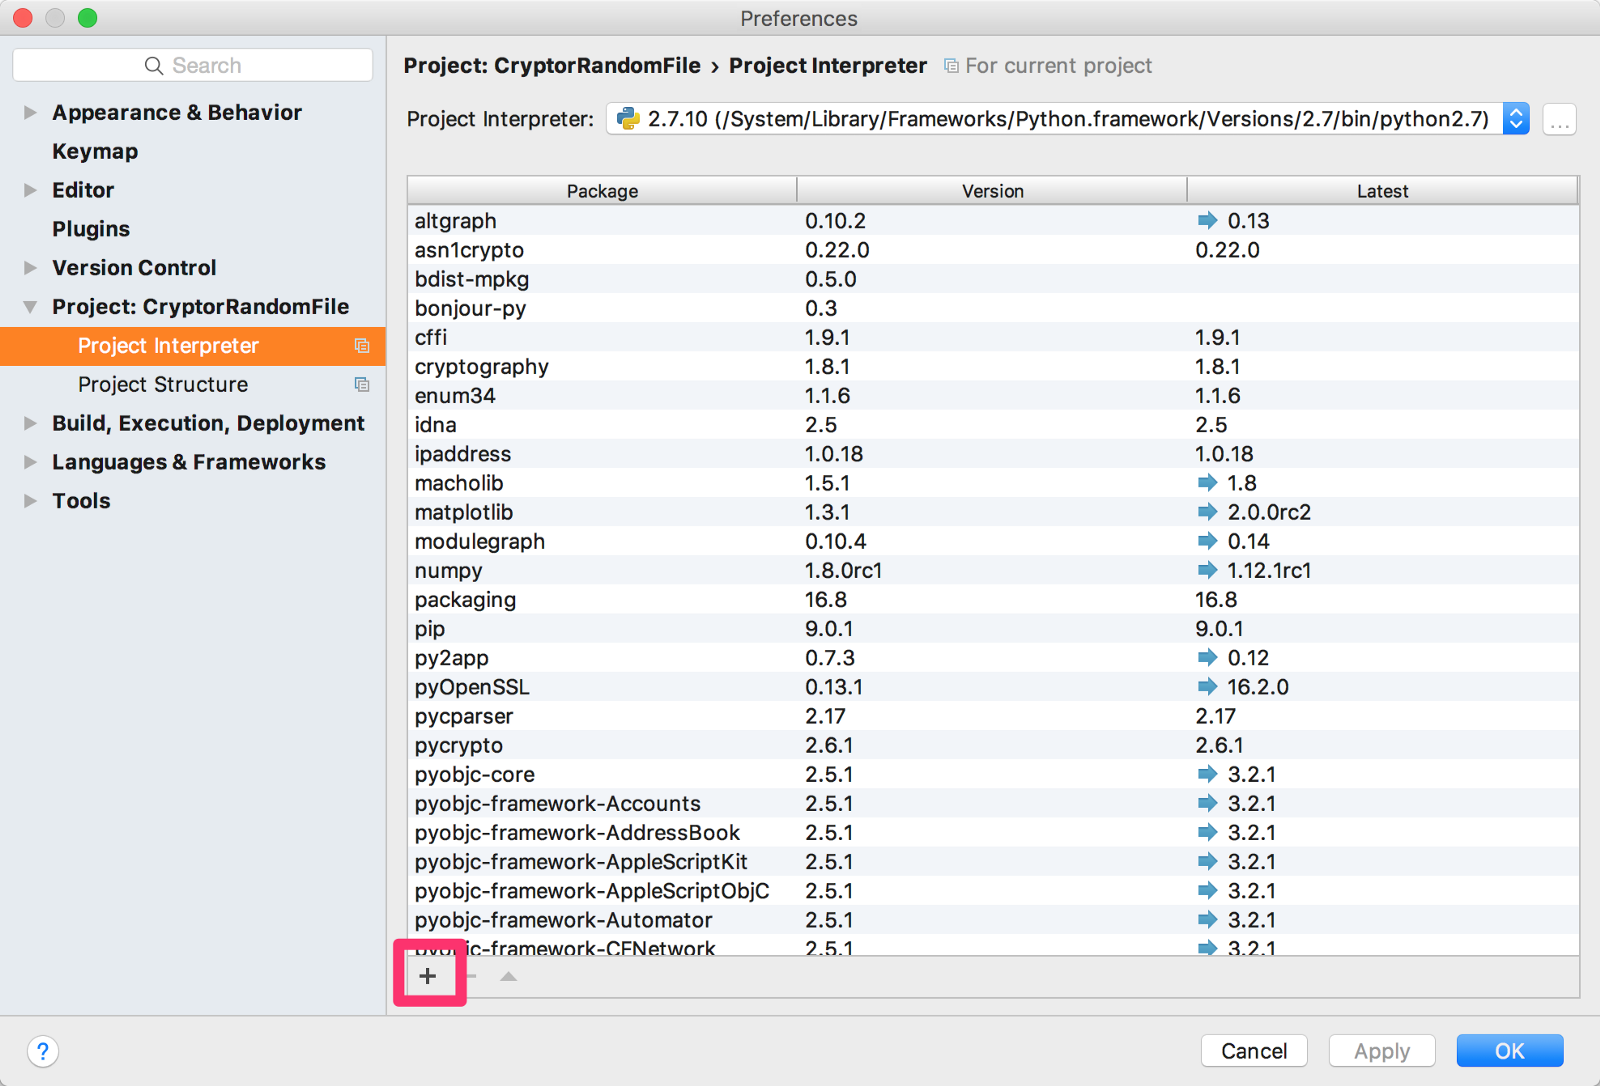
\includegraphics[scale=0.2]{image/PyCharm2.png}
	\end{center}
\end{figure}

輸入要加入的package name

\begin{figure}[ht]
	\begin{center}
		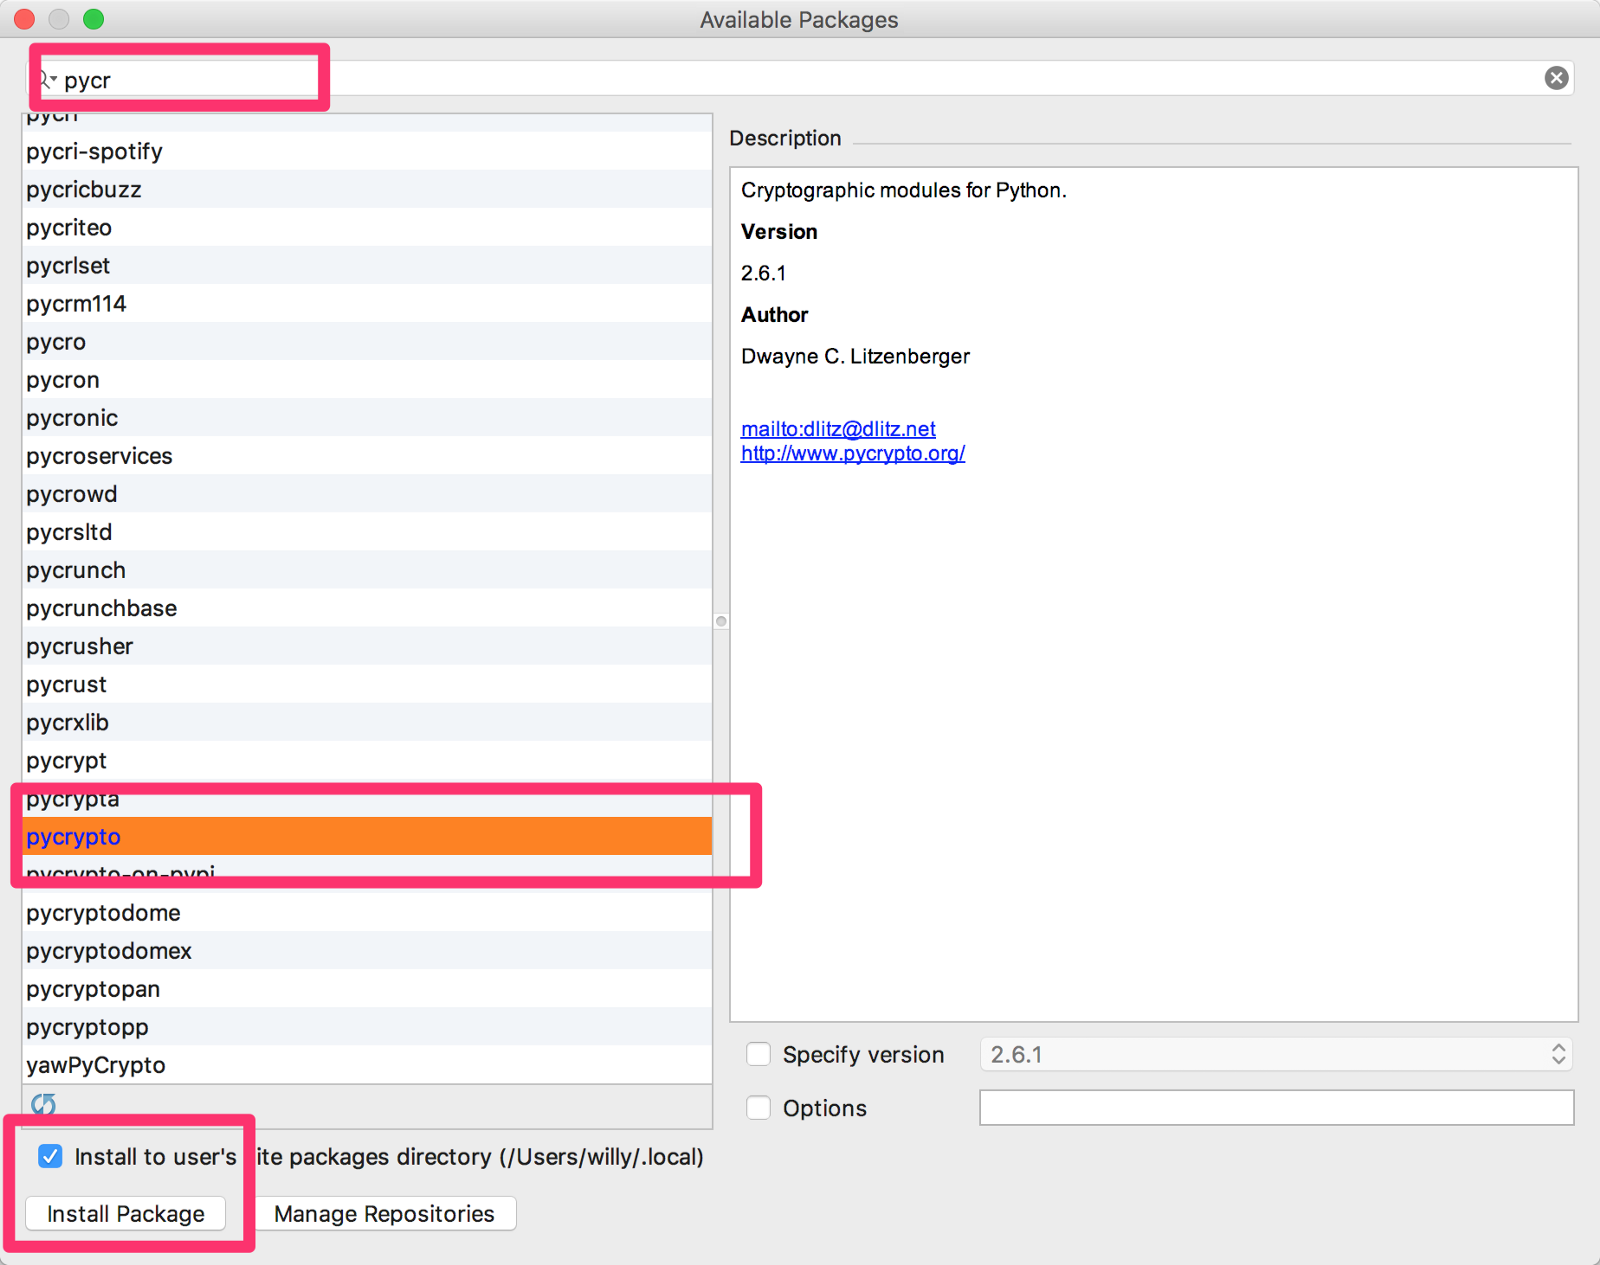
\includegraphics[scale=0.2]{image/PyCharm3.png}
	\end{center}
\end{figure}

}

\newpage % 新一頁
\section{PyCrypto}

\subsection{PyCrypto AES-256 ECB}
{

\begin{lstlisting}[language=Python]
# -*- coding: utf-8 -*-

from __future__ import absolute_import, division, unicode_literals

import os
from Crypto.Cipher import AES

_KEY = os.urandom(32)		# 設定Key
_BlockSize = AES.block_size	# Block Size

#padding
_Pad = lambda s: s + (_BlockSize - len(s) % _BlockSize) * chr(_BlockSize - len(s) % _BlockSize)
_Unpad = lambda s : s[0:-ord(s[-1])]

# 使用ECB加密
def aes_encrypt(data):
    cryptor = AES.new(_KEY, AES.MODE_ECB)
    return cryptor.encrypt(_Pad(data))

# 使用ECB解密
def aes_decrypt(data):
    cryptor = AES.new(_KEY, AES.MODE_ECB)
    return _Unpad(cryptor.decrypt(data))
\end{lstlisting}
}

\subsection{PyCrypto AES-256 CBC}
{
\begin{lstlisting}[language=Python]
# -*- coding: utf-8 -*-

from __future__ import absolute_import, division, unicode_literals

import os
from Crypto.Cipher import AES

_IV = os.urandom(16)		# 產生隨機亂數IV
_KEY = os.urandom(32)		# 設定Key
_BlockSize = AES.block_size	# Block Size

#padding
_Pad = lambda s: s + (_BlockSize - len(s) % _BlockSize) * chr(_BlockSize - len(s) % _BlockSize)
_Unpad = lambda s : s[0:-ord(s[-1])]

# 使用CBC加密
def aes_encrypt(data):
    cryptor = AES.new(_KEY, AES.MODE_CBC, _IV)
    return cryptor.encrypt(_Pad(data))

# 使用CBC解密
def aes_decrypt(data):
    cryptor = AES.new(_KEY, AES.MODE_CBC, _IV)
    return _Unpad(cryptor.decrypt(data))
\end{lstlisting}
}

\subsection{PyCrypto AES-256 CTR}
{
\begin{lstlisting}[language=Python]
# -*- coding: utf-8 -*-

from __future__ import absolute_import, division, unicode_literals

import os
from Crypto.Cipher import AES

_IV = os.urandom(16)		# 產生隨機亂數IV
_KEY = os.urandom(32)		# 設定Key
_COUNTER = os.urandom(16)
_BlockSize = AES.block_size # Block Size

#padding
_Pad = lambda s: s + (_BlockSize - len(s) % _BlockSize) * chr(_BlockSize - len(s) % _BlockSize)
_Unpad = lambda s : s[0:-ord(s[-1])]

# 使用CTR加密
def aes_encrypt(data):
    cryptor = AES.new(_KEY, AES.MODE_CTR, counter=lambda: _COUNTER)
    return cryptor.encrypt(_Pad(data))

# 使用CTR解密
def aes_decrypt(data):
    cryptor = AES.new(_KEY, AES.MODE_CTR, counter=lambda: _COUNTER)
    return _Unpad(cryptor.decrypt(data))
\end{lstlisting}
}

\subsection{PyCrypto RSA-2048}
{
\begin{lstlisting}[language=Python]
	
\end{lstlisting}
}

\subsection{PyCrypto SHA-512}
{
\begin{lstlisting}[language=Python]
# -*- coding: utf-8 -*-
from __future__ import absolute_import, division, unicode_literals

from Crypto.Hash import SHA512

def hashSHA512(data):
    hash = SHA512.new()
    hash.update(data)
    return hash.hexdigest()
\end{lstlisting}
}

\newpage % 新一頁
\section{Cryptography}

\subsection{Cryptography AES-256 ECB}
{
\begin{lstlisting}[language=Python]
import os
from cryptography.hazmat.primitives.ciphers import Cipher, algorithms, modes
from cryptography.hazmat.backends import default_backend

backend = default_backend()
_KEY = os.urandom(32)	# 設定Key
_BlockSize = 16	        # Block Size

#padding
_Pad = lambda s: s + (_BlockSize - len(s) % _BlockSize) * chr(_BlockSize - len(s) % _BlockSize)
_Unpad = lambda s : s[0:-ord(s[-1])]

# 使用ECB加密
def aes_encrypt(data):
    cipher = Cipher(algorithms.AES(_KEY), modes.ECB(), backend=backend)
    encryptor = cipher.encryptor()
    ciphertext = encryptor.update(_Pad(data))
    return ciphertext

# 使用ECB解密
def aes_decrypt(data):
    cipher = Cipher(algorithms.AES(_KEY), modes.ECB(), backend=backend)
    decryptor = cipher.decryptor()
    plaintext = _Unpad(decryptor.update(data))  # + decryptor.finalize()
    return plaintext
\end{lstlisting}
}

\subsection{Cryptography AES-256 CBC}
{
\begin{lstlisting}[language=Python]
import os
from cryptography.hazmat.primitives.ciphers import Cipher, algorithms, modes
from cryptography.hazmat.backends import default_backend

backend = default_backend()
_IV = os.urandom(16)    # 產生隨機亂數IV
_KEY = os.urandom(32)	# 設定Key
_BlockSize = 16	        # Block Size

#padding
_Pad = lambda s: s + (_BlockSize - len(s) % _BlockSize) * chr(_BlockSize - len(s) % _BlockSize)
_Unpad = lambda s : s[0:-ord(s[-1])]

# 使用CBC加密
def aes_encrypt(data):
    cipher = Cipher(algorithms.AES(_KEY), modes.CBC(_IV), backend=backend)
    encryptor = cipher.encryptor()
    ciphertext = encryptor.update(_Pad(data))
    return ciphertext

# 使用CBC解密
def aes_decrypt(data):
    cipher = Cipher(algorithms.AES(_KEY), modes.CBC(_IV), backend=backend)
    decryptor = cipher.decryptor()
    plaintext = _Unpad(decryptor.update(data))
    return plaintext
\end{lstlisting}
}

\subsection{Cryptography AES-256 CTR}
{
\begin{lstlisting}[language=Python]
import os
from cryptography.hazmat.primitives.ciphers import Cipher, algorithms, modes
from cryptography.hazmat.backends import default_backend

backend = default_backend()
_IV = os.urandom(16)    # 產生隨機亂數IV
_KEY = os.urandom(32)	# 設定Key
_BlockSize = 16	        # Block Size

#padding
_Pad = lambda s: s + (_BlockSize - len(s) % _BlockSize) * chr(_BlockSize - len(s) % _BlockSize)
_Unpad = lambda s : s[0:-ord(s[-1])]

# 使用CTR加密
def aes_encrypt(data):
    cipher = Cipher(algorithms.AES(_KEY), modes.CTR(_IV), backend=backend)
    encryptor = cipher.encryptor()
    ciphertext = encryptor.update(_Pad(data))
    return ciphertext

# 使用CTR解密
def aes_decrypt(data):
    cipher = Cipher(algorithms.AES(_KEY), modes.CTR(_IV), backend=backend)
    decryptor = cipher.decryptor()
    plaintext = _Unpad(decryptor.update(data))
    return plaintext
\end{lstlisting}
}

\subsection{Cryptography RSA-2048}
{
\begin{lstlisting}[language=Python]
	
\end{lstlisting}
}

\subsection{Cryptography SHA-512}
{
\begin{lstlisting}[language=Python]
from cryptography.hazmat.primitives import hashes
from cryptography.hazmat.backends import default_backend

backend = default_backend()

def hashSHA512(data):
    digest = hashes.Hash(hashes.SHA512(), backend=default_backend())
    digest.update(data)
    return digest.finalize()
\end{lstlisting}
}

\newpage % 新一頁
\section{PyCrypto 與 Cryptography 速度的比較}
利用Python隨機產生一個大小為512+7byte的字串檔案
並且丟到每一個加解密演算法計算時間
\subsection{隨機產生字串檔案}
{
\begin{lstlisting}[language=Python]
# -*- coding: utf-8 -*-
import random, string

# 隨機產生大小為size的字串檔案
def generateStringFile(size):
    text = ''.join(random.choice(string.ascii_letters + string.digits) for x in range(size))
    file = open('RandomString.txt', 'wb')
    file.write(text)
\end{lstlisting}
}

\subsection{AES-256 ECB}
{
\begin{lstlisting}[language=Python]
# PyCrypto_AES_256_ECB
print ('PyCrypto_AES_256_ECB')
start = time.time()
encrypt = PyCrypto_AES_256_ECB.aes_encrypt(plaintext)
end = time.time()
elapsed = end - start
print ('Time taken: ' + str(elapsed) + 'seconds.')

# Cryptography_AES_256_ECB
print ('Cryptography_AES_256_ECB')
start = time.time()
encrypt = Cryptography_AES_256_ECB.aes_encrypt(plaintext)
end = time.time()
elapsed = end - start
print ('Time taken: ' + str(elapsed) + 'seconds.')
\end{lstlisting}
輸出的結果為
\newline PyCrypto AES256 ECB
Time taken: 8.11543488503seconds.
\newline Cryptography AES256 ECB
Time taken: 2.48533296585seconds.
}

\subsection{AES-256 CBC}
{
\begin{lstlisting}[language=Python]
# PyCrypto_AES_256_CBC
print ('PyCrypto_AES_256_CBC')
start = time.time()
encrypt = PyCrypto_AES_256_CBC.aes_encrypt(plaintext)
end = time.time()
elapsed = end - start
print ('Time taken: ' + str(elapsed) + 'seconds.')

# Cryptography_AES_256_CBC
print ('Cryptography_AES_256_CBC')
start = time.time()
encrypt = Cryptography_AES_256_CBC.aes_encrypt(plaintext)
end = time.time()
elapsed = end - start
print ('Time taken: ' + str(elapsed) + 'seconds.')
\end{lstlisting}
輸出的結果為
\newline PyCrypto AES256 CBC
Time taken: 6.45398807526seconds.
\newline Cryptography AES256 CBC
Time taken: 3.81276679039seconds.
}

\subsection{AES-256 CTR}
{
\begin{lstlisting}[language=Python]
# PyCrypto_AES_256_CTR
print ('PyCrypto_AES_256_CTR')
start = time.time()
encrypt = PyCrypto_AES_256_CTR.aes_encrypt(plaintext)
end = time.time()
elapsed = end - start
print ('Time taken: ' + str(elapsed) + 'seconds.')

# Cryptography_AES_256_CTR
print ('Cryptography_AES_256_CTR')
start = time.time()
encrypt = Cryptography_AES_256_CTR.aes_encrypt(plaintext)
end = time.time()
elapsed = end - start
print ('Time taken: ' + str(elapsed) + 'seconds.')
\end{lstlisting}
輸出的結果為
\newline PyCrypto AES256 CTR
Time taken: 21.1867408752seconds.
\newline Cryptography AES256 CTR
Time taken: 2.08338999748seconds.
}

\subsection{RSA-2048}
{
\begin{lstlisting}[language=Python]
	
\end{lstlisting}
輸出的結果為
}

\subsection{SHA-512}
{
\begin{lstlisting}[language=Python]
# PyCrypo_SHA_512
print ('PyCrypo_SHA_512')
start = time.time()
hash = PyCrypo_SHA_512.hashSHA512(plaintext)
end = time.time()
elapsed = end - start
print ('Time taken: ' + str(elapsed) + 'seconds.')

# Cryptography_SHA_512
print ('Cryptography_SHA_512')
start = time.time()
hash = Cryptography_SHA_512.hashSHA512(plaintext)
end = time.time()
elapsed = end - start
print ('Time taken: ' + str(elapsed) + 'seconds.')	
\end{lstlisting}
輸出的結果為
\newline PyCrypo SHA512
Time taken: 2.17035508156seconds.
\newline Cryptography SHA512
Time taken: 1.27641797066seconds.
}

\end{document}